\section{Game Concept Development}

This section describes the process of coming up with a concept for the game, as well as where inspiration came from. Initially the group considered the power industry in Norway. Thereafter two quite different game concepts were developed and presented to the customer.

\subsection{The Power Industry}

\begin{wrapfigure}{r}{40mm}
  \begin{center}
  
\includegraphics[scale=0.5]{pictures/water_generator.png}
  \end{center}
\end{wrapfigure}

In Norway 99\% of all power production is generated through hydropower. Hydropower is generated when pressurized water is used to drive a turbine which turns the energy of the water into electricity. When electricity has been produced, it passes through the transformer where it is stepped up to high voltage. Then it is sent onto the power grid. Hydropower is pollution-free and renewable. Because water is often stored in reservoirs, it is also very flexible; electricity can be produced when demand is high. \cite{statkraftVannkraft}

\subsection{The First Game Concept}

During the first meeting with the customer, it was clear that they did not have a very specific idea of what the game should contain beyond what the project description said. The product description says that the game should be focused around controlling power production from hydro plants trough a power grid to the customers, but it could also be centered around something else as long as the theme of hydro power was kept. The conclusion in the first customer meeting, concerning the concept, was that most importantly the game should be fun and something users would want to play. This
lead the group to a phase in which different options for a game concept were considered.

The group's first idea was inspired by games that have a simple concept interface, but that are still fun and addictive, as those games often turns out to be the most popular, e.g. Tetris. In brief the first concept the group came up with was a simple, level based 2d game, where the goal is to serve all customers (nodes) with power produced from the power station
(Helgelandskraft). The nodes are scattered around the screen, and the player draws a line from node to node without lifting his or her finger. There is not unlimited power, so the player needs to find the shortest path to deliver
power to all nodes. If the power station runs out of power before every node is served, the player loose and needs to start the level from scratch.

This idea was presented in the second customer meeting. The customer liked it, but was also unsure whether it was too abstract from what a power plant company actually do. 

\begin{figure}
	\center
	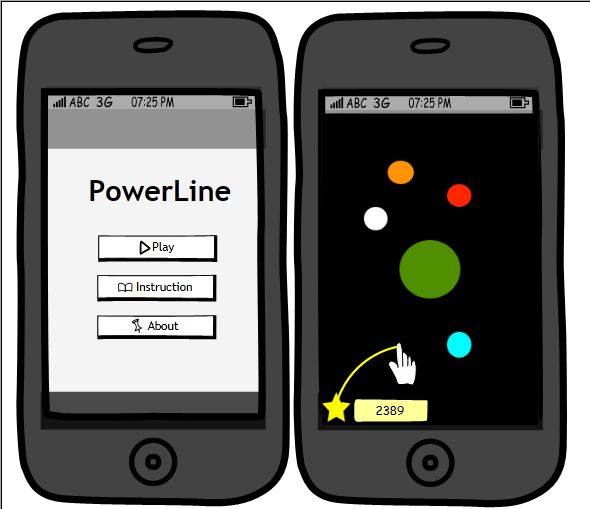
\includegraphics[scale=0.75]{pictures/Skisse}
	\caption{Sketch of the first game concept.}
\end{figure}

\subsection{The Final Game Concept}

Following this meeting the customer was asked to come up with a more specific concept of their own, and the group would also look at other options for a game concept. The second game concept had more base in reality. Briefly explained, the player is in charge of the electric utility in town and has the responsibility of supplying the inhabitants and local industry with electricity by building power plants and power lines. When brainstorming for this concept the group began to look to construction and management simulation games, as this could be a good way to present an industry and how it works as well as create a fun and challenging game. At the following customer meeting both the groups and the customers ideas were presented. The final game concept was decided during this meeting. A more detailed description of the final game concept can be found in Chapter \ref{chap:gameconsept} Game Concept. The customer was happy with this concept as it was closer to what the product description explained and more realistic.

	\begin{figure}[H]
	\centering
		\subfigure{
			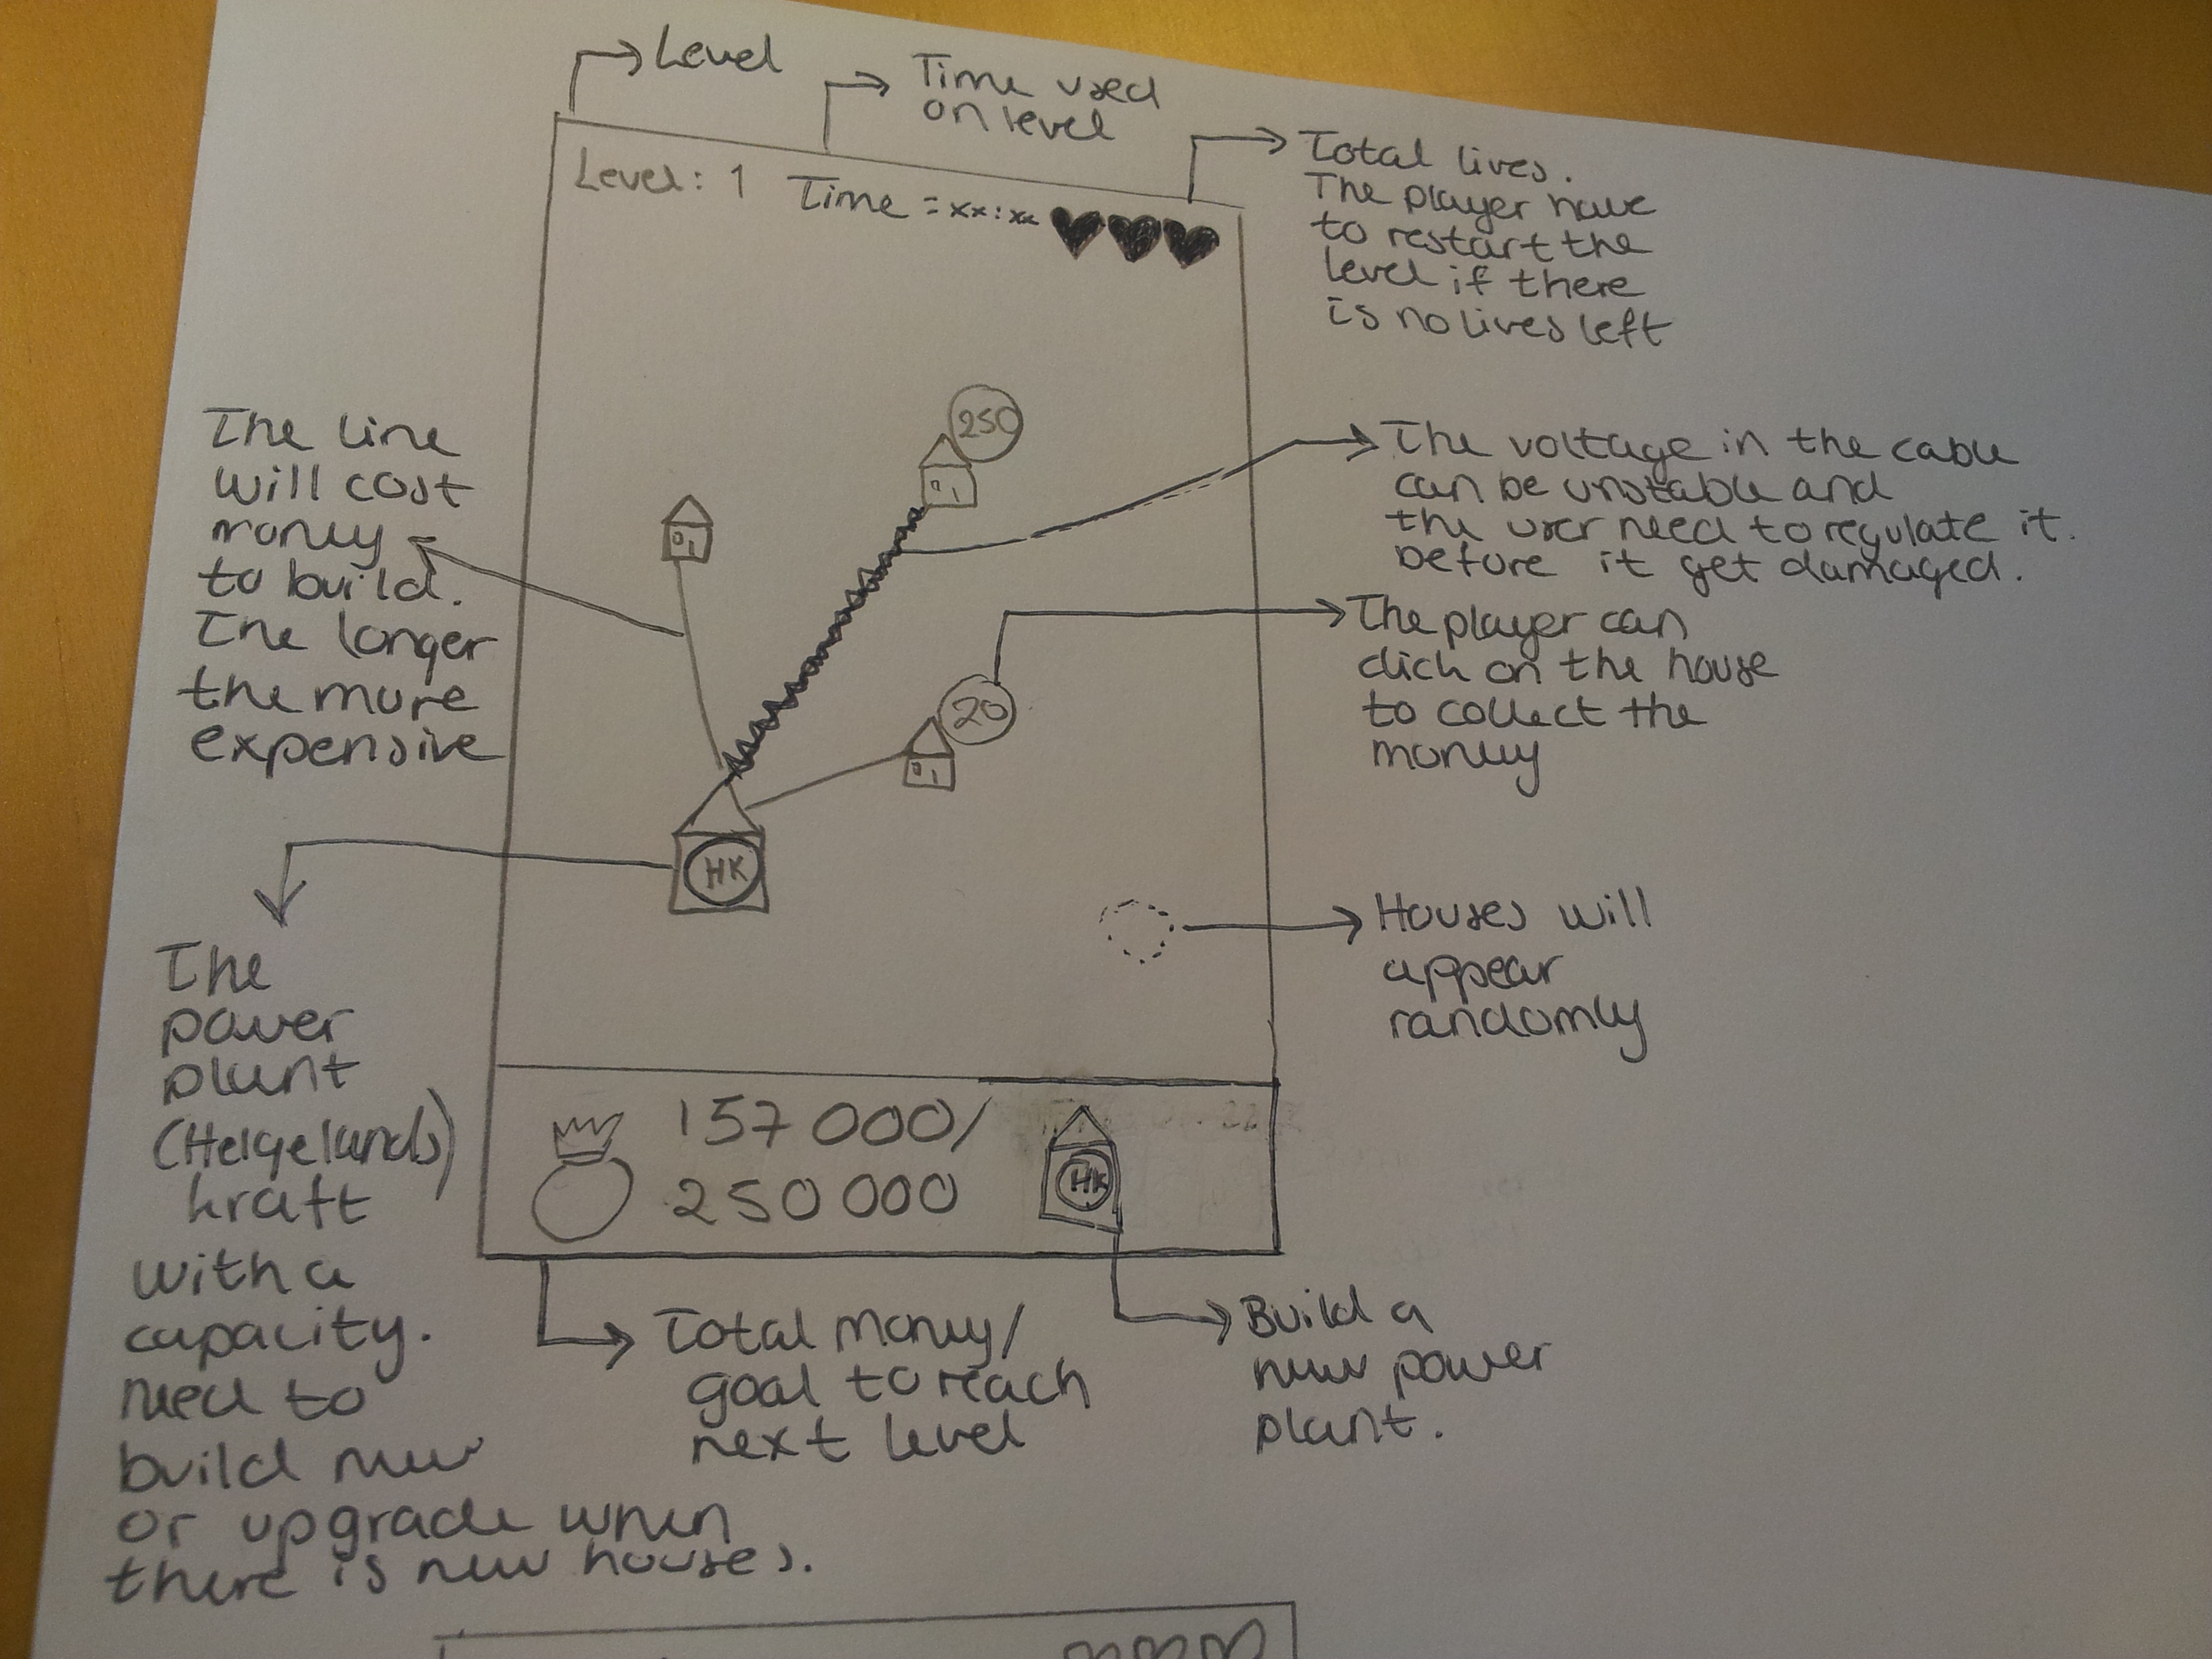
\includegraphics[scale=0.05]{pictures/gameConcept1}
		}
		\subfigure{
			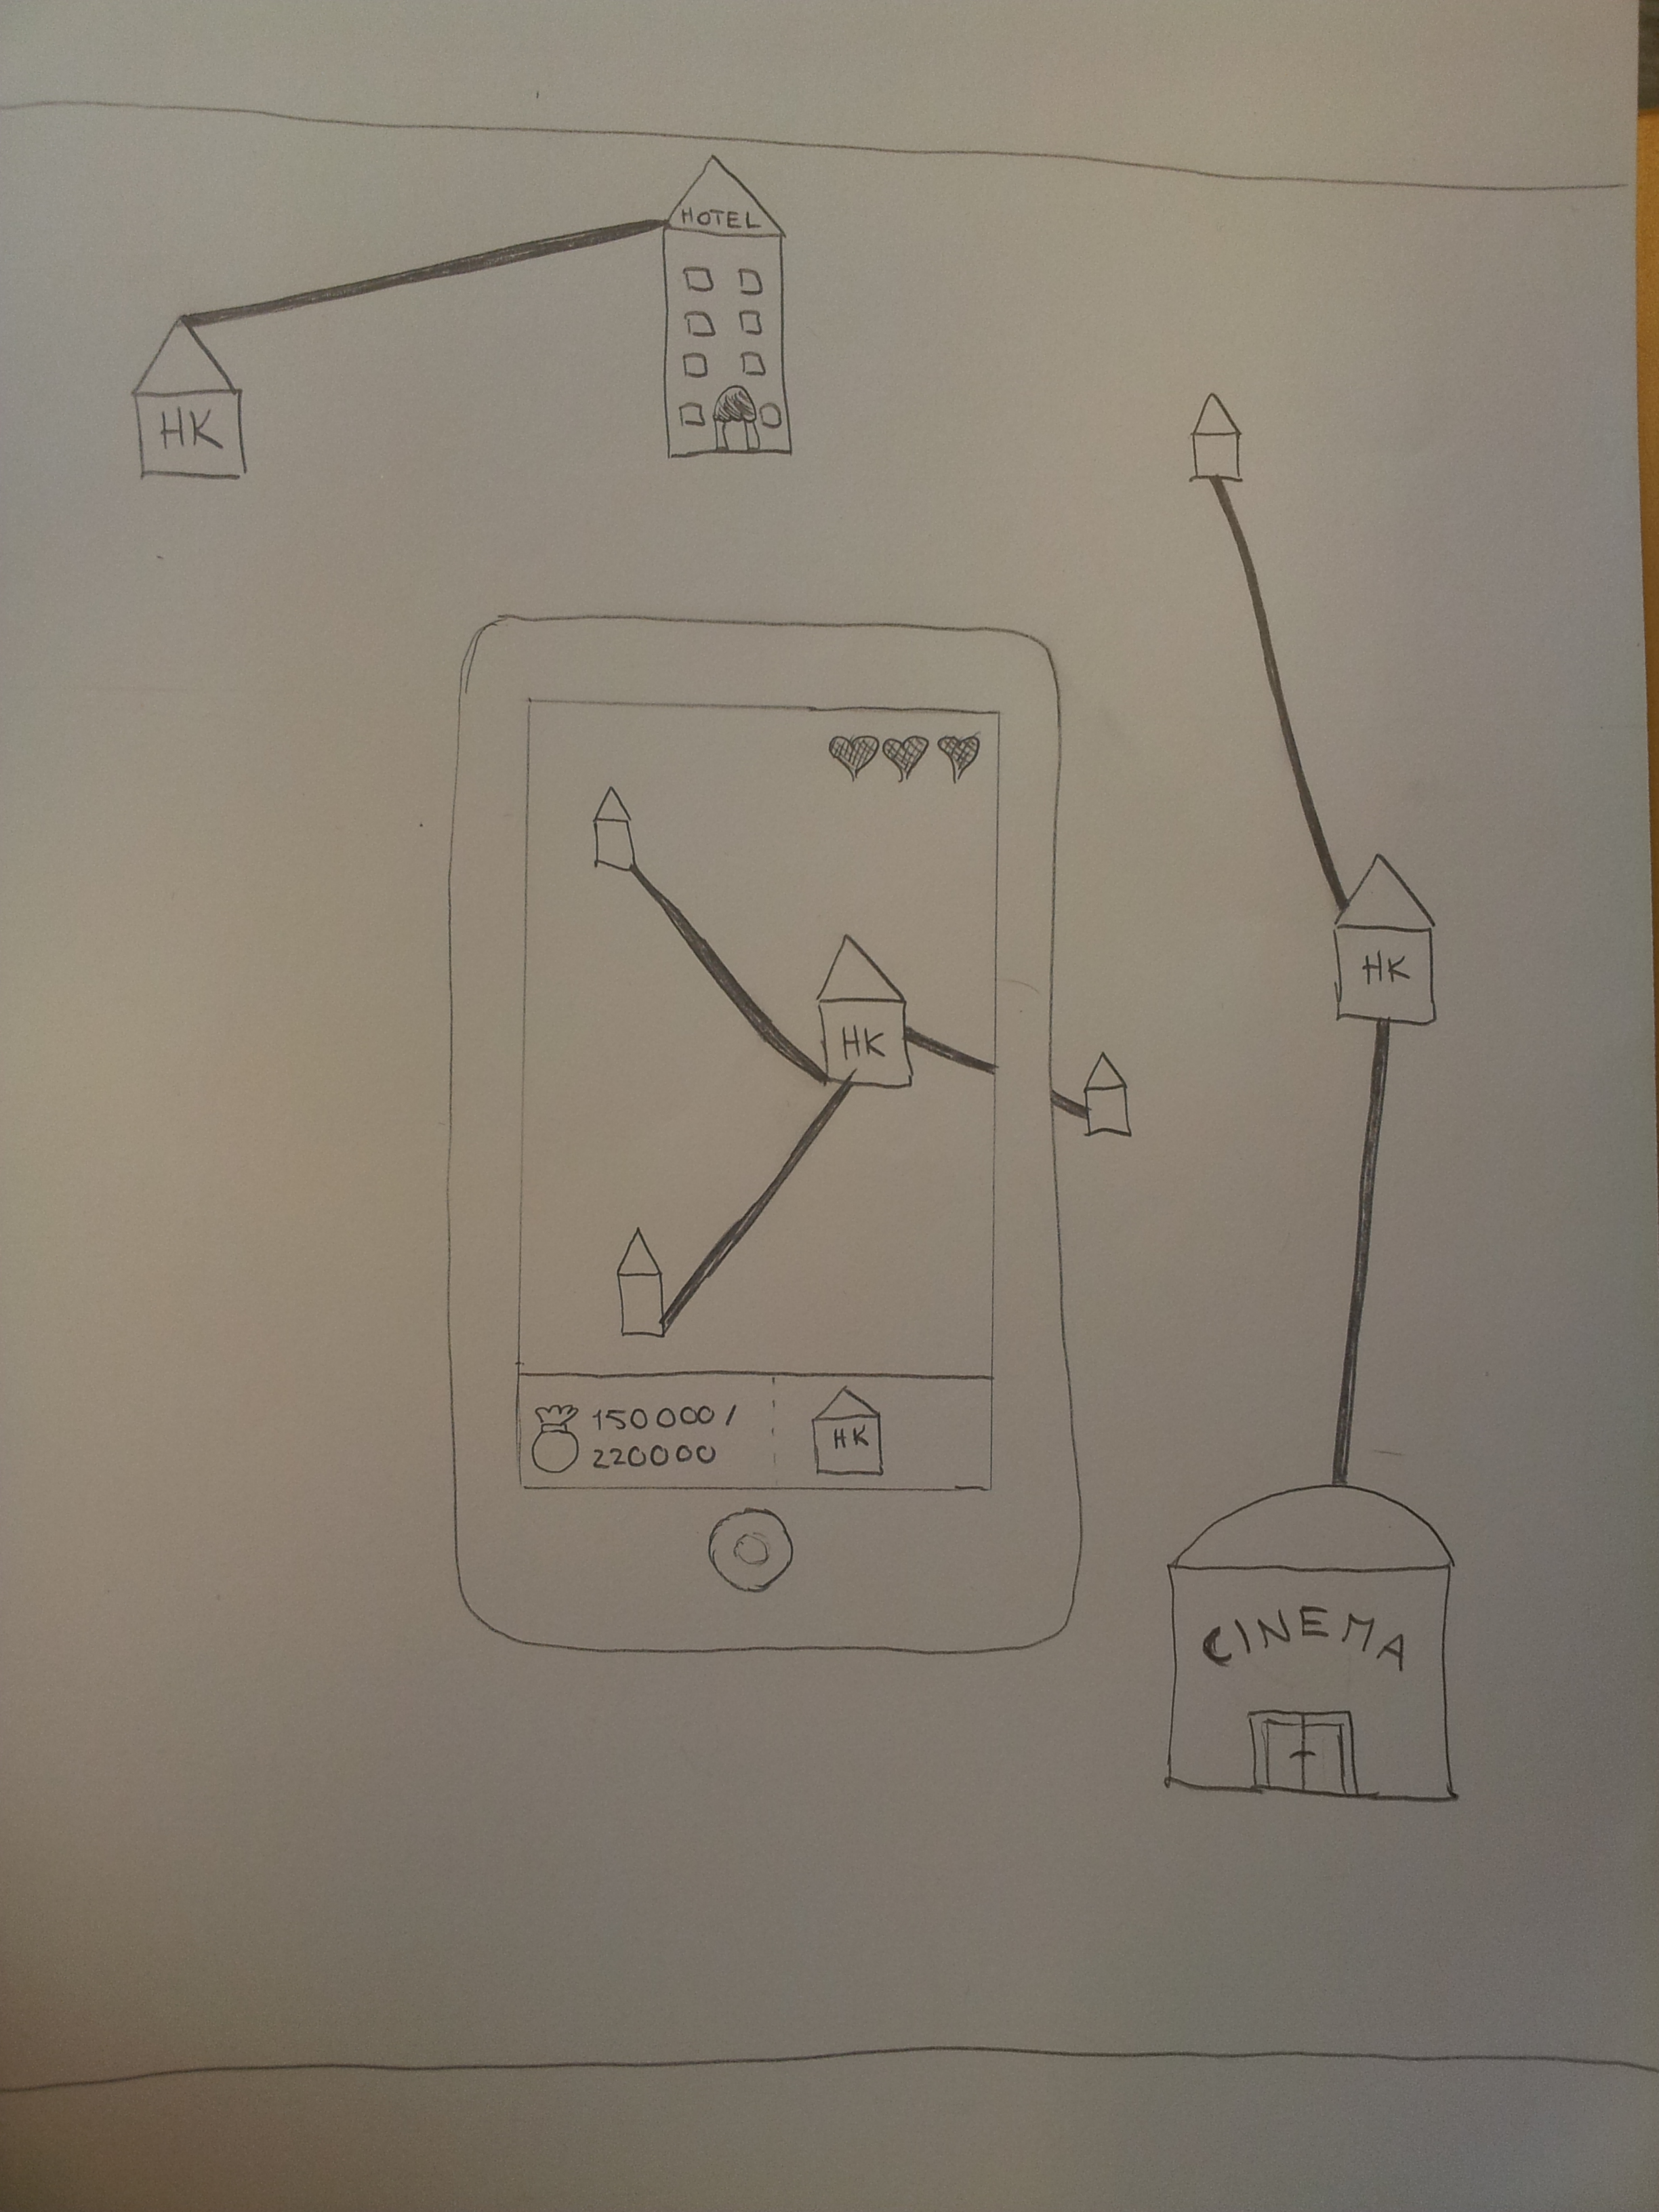
\includegraphics[scale=0.05]{pictures/gameConcept2}
		}
		\caption{Game concept development}
	\end{figure}

\subsection{Similar Game Concepts}

{\bf Construction and management simulation games}

Construction and management simulation games, hereafter called CMS games, are based on building, managing and expanding virtual communities or projects with limited resources. CMS games have been developed since the 1980s and continue to be popular to this day. SimCity, which was released in 1989 and is considered to be the first CMS game to be highly successful, has spawned numerous successors, the last one released this year. \cite{wikiCMS}

{\bf Megapolis}

One specific game that the group took a closer look at was the Megapolis game developed by Social Quantum for the iPhone and iPad. This is a construction and management simulation game in which the player builds his own virtual city. As the person in charge of the city the player needs to manage the finances of the city, provide it with water and electricity, and develop infrastructure such as airports and power plants. The goal is to keep expanding the city, unlock new tasks and rewards and build the most impressive city. \cite{megapolis}

\begin{figure}[H]
	\centering
	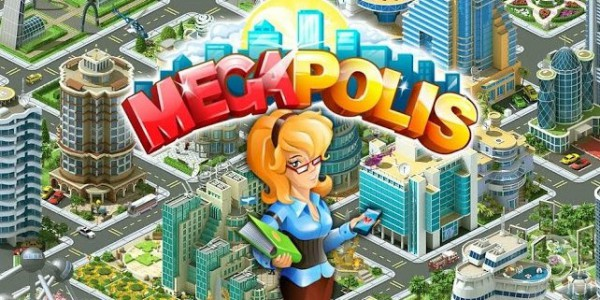
\includegraphics[width=\textwidth]{pictures/megapolis.jpg}
	\caption{Game: Megapolis}
\end{figure}

The group found a number of other CMS games when searching through AppStore and GooglePlay, but none in which power production and power supply were a major part of the game. This does however prove that there is an interest for games
with elements of CMS.

Finding games with elements of power supply and production proved to be more difficult.

\subsection{Conclusions}

The group decided to develop a construction and management game, dubbed Power Supply. CMS games are very popular, both as more dedicated games like SimCity and casual games like Megapolis, and a point the customer was very clear about was that they primarily wanted people to play the game. Developing a game in a genre that is widely popular made sense. It is also a genre that the group members are familiar with playing. The final game concept is described in Chapter \ref{chap:gameconsept} Game Concept.
